% !TeX program = pdflatex
% !TeX encoding = UTF-8
%=======================================================================
%  GRIS-NOT-001  ·  Plantilla de notas rápidas para la memoria
%  Proyecto 00503 - Generator inspection robotic system · Mecanalisis
%  Identidad: GRIS-IDENTIDAD-001 v1.4
%-----------------------------------------------------------------------
%  CÓMO USARLA (en 3 pasos)
%
%   1. Copiá este archivo con el código de la nota:
%         memoria/notas/02489-00-MC007.tex
%      El número (###) es correlativo: mirá la última nota y sumá uno.
%
%   2. Completá los cuatro datos del bloque «DATOS DE LA NOTA».
%
%   3. Escribí:
%        · Resultados (obligatorio, siempre primero): lo que se sabe
%          ahora que antes no se sabía. Frases cortas, con números.
%        · El resto es libre. Usá los títulos que te sirvan, o ninguno.
%
%   Compilar:  pdflatex 02489-00-MC007.tex
%   En Overleaf: subí el .tex y logo-gris.pdf.
%
%  LOGO: se usa «logo-gris.pdf» (GRIS-LOGO-003, reducido) de esta carpeta
%  o de ../plantilla/. Si falta, se escribe «GRIS» como marcador.
%=======================================================================
\documentclass[11pt,a4paper]{article}

%=======================================================================
%  DATOS DE LA NOTA  ← lo único que hay que tocar arriba
%=======================================================================
\newcommand{\codigo}{02489-00-MC005}          % 02489-00-MC###
\newcommand{\titulo}{Selección del solenoide del impactador}
\newcommand{\autor}{Matías Gaviño}
\newcommand{\fecha}{24/09/2026}                    % o p. ej. {24/09/2026}

%=======================================================================
%  ESTILO  (no hace falta tocar nada de aquí hasta \begin{document})
%=======================================================================
\usepackage[T1]{fontenc}
\usepackage[utf8]{inputenc}
\usepackage[spanish,es-noshorthands,es-tabla]{babel}
\usepackage{lmodern}
\usepackage[a4paper,top=3.0cm,bottom=2.4cm,left=2.4cm,right=2.4cm,
            headheight=20pt,headsep=1.2cm,footskip=1.1cm]{geometry}
\usepackage{microtype}
\usepackage{xcolor}
\usepackage{graphicx}
\usepackage{booktabs}
\usepackage{array}
\usepackage{enumitem}
\usepackage{titlesec}
\usepackage{fancyhdr}
\usepackage{caption}
\usepackage{amsmath}
\usepackage{amssymb}
\usepackage{float}
\usepackage{longtable}
\usepackage{xurl}
\usepackage[hidelinks]{hyperref}

% --- colores -----------------------------------------------------------
\definecolor{gris-naranja}{HTML}{FF7A00}   % naranja institucional
\definecolor{tinta}{HTML}{1E2328}
\definecolor{gris-medio}{HTML}{6B7280}
\definecolor{gris-linea}{HTML}{DADDE1}
\color{tinta}

\hypersetup{pdftitle={\codigo\ -- \titulo}, pdfauthor={\autor},
            colorlinks=true, linkcolor=tinta, urlcolor=tinta}

% --- logo ---------------------------------------------------------------
\graphicspath{{./}{../plantilla/}{plantilla/}{02489-00-MC005/figuras/}}
\newcommand{\logogris}{%
  \IfFileExists{logo-gris.pdf}
    {
\includegraphics[height=16pt]{logo-gris.pdf}}
    {\IfFileExists{../plantilla/logo-gris.pdf}
      {
\includegraphics[height=16pt]{../plantilla/logo-gris.pdf}}
      {{\fontsize{18}{18}\selectfont\bfseries\sffamily\color{gris-naranja}GRIS}}}}

% --- tipografía del cliente (código documental) --------------------------
% Geogrotesque no es libre; se usa Roboto Condensed Bold, que viene con
% TeX Live y Overleaf y tiene el mismo aire que el logo.
\newcommand{\fuentecliente}{\fontfamily{Roboto-TLF}\fontseries{bc}\selectfont}

% --- encabezado y pie ---------------------------------------------------
\pagestyle{fancy}
\fancyhf{}
\renewcommand{\headrulewidth}{0.4pt}
\renewcommand{\headrule}{\vspace{3pt}{\color{gris-linea}\hrule height \headrulewidth}}
\fancyhead[L]{\logogris}
\fancyhead[R]{{\fuentecliente\fontsize{12}{12}\selectfont\color{gris-medio}\codigo}}
\fancyfoot[R]{\footnotesize\color{gris-medio}\thepage}

% --- títulos numerados ----------------------------------------------------
\setcounter{secnumdepth}{2}
\titleformat{\section}{\large\bfseries}{\thesection}{0.8em}{}
\titleformat{\subsection}{\normalsize\bfseries}{\thesubsection}{0.8em}{}
\titlespacing*{\section}{0pt}{16pt}{5pt}
\titlespacing*{\subsection}{0pt}{11pt}{3pt}

% --- texto ------------------------------------------------------------------
\setlength{\parindent}{0pt}
\setlength{\parskip}{6pt}
\linespread{1.05}
\setlist{topsep=2pt, itemsep=2pt, parsep=0pt, leftmargin=1.2em}
\setlist[itemize]{label={\raisebox{0.15ex}{\small$\bullet$}}}
\captionsetup{font={small,color=gris-medio}, labelfont=bf, skip=5pt}
\renewcommand{\arraystretch}{1.25}

% --- cabecera de la nota ------------------------------------------------------
\newcommand{\cabecera}{%
  \thispagestyle{fancy}%
  {\fontsize{20}{24}\selectfont\bfseries\titulo\par}%
  \vspace{5pt}%
  {\small\color{gris-medio}\fecha\quad·\quad\autor\par}%
  \vspace{6pt}}

% --- ayudas opcionales --------------------------------------------------------
% \figura{archivo}{ancho}{pie}
\newcommand{\figura}[3]{%
  \begin{figure}[htbp]\centering
    \includegraphics[width=#2\linewidth]{#1}\caption{#3}
  \end{figure}}

%=======================================================================
\newcommand{\hoja}[2]{\fbox{\includegraphics[width=#1\linewidth]{#2}}}
\setlength{\fboxrule}{0.3pt}\setlength{\fboxsep}{0pt}
\newcommand{\ok}{\textbf{sí}}
\newcommand{\no}{\textbf{no}}

\begin{document}
\cabecera

%-----------------------------------------------------------------------
%  RESULTADOS  (siempre primero, lo único obligatorio)
%-----------------------------------------------------------------------
\section{Resultados}
\textbf{El criterio que decide es el trabajo bajo la curva fuerza--carrera \emph{sin llegar al tope interno}}
(impacto a $x_\mathrm{imp}=0{,}5$~mm del tope), no la fuerza de retención. Todas las curvas se extrajeron de
las hojas de datos oficiales (anexo~\ref{sec:anexo}) con \texttt{02489-00-MC005/calculo.py}; los valores son
cotas superiores estáticas ($\eta=1$).

\begin{table}[H]\centering\footnotesize\setlength{\tabcolsep}{2.6pt}
\begin{tabular}{l l r r r l l}
\toprule
Candidato & Envolvente [mm] & $W_\mathrm{útil}$ [mJ] & Planitud & $S_{0,1}$ [\%] & Vida & Veredicto\\
\midrule
Takaha CA0425   & 10$\times$12$\times$24,8          & 6,8 & 1,3  & 4,6  & no publica   & ensayar\\
Takaha CA0422   & 9,8$\times$10,8$\times$21,3       & 6,0 & 1,5  & 5,2  & no publica   & \textbf{elegido (10$\times$10)}\\
Geeplus 144C    & $\varnothing$13,8$\times$21       & 9,9 & 6,0  & 7,5  & $>$5~M       & \textbf{elegido si $\varnothing$14}\\
Geeplus 141C    & $\varnothing$13,8$\times$13,7     & 4,4 & 13,7 & 12,8 & $>$5~M       & justo; cotizar modificado\\
Ledex B12P (10\,\% ED) & 16$\times$8,1$\times$10,2  & 4,2 & 3,8  & 7,0  & no publica   & consultar vida\\
Geeplus RD-A420 & 21,4$\times$10,8$\times$9,8       & 4,0 & 3,3  & 6,4  & $>$250~k     & descartado\\
Geeplus 110C    & $\varnothing$11,3$\times$13,3     & 1,3 & 5,6  & 14,8 & $>$5~M       & descartado\\
\bottomrule
\end{tabular}
\caption{Resumen. Planitud $=F(x_\mathrm{imp})/F(x_\mathrm{ini})$; $S_{0,1}$: cambio de energía si la cuña se
corre 0,1~mm. Objetivo: 3--5~mJ de energía cinética.}
\end{table}

\begin{itemize}
  \item \textbf{Takaha CA0422/CA0425 tienen la curva más plana de la lista} (la fuerza varía solo $\times$1,3--1,5
        en 2,5~mm) y dan \textbf{6,0 y 6,8~mJ} sin tocar el tope, con la menor sensibilidad a la posición
        ($\approx$5\,\% cada 0,1~mm). Entran en la sección de 10$\times$11~mm y cuestan USD~9.
        \textbf{Tres pendientes:} son de \emph{tracción}, la hoja no publica vida útil ni la masa del émbolo
        (estimada en $\approx$2~g).
  \item \textbf{El Geeplus 141C no tiene energía «sobrada»:} da 8,9~mJ hasta el tope, pero \textbf{4,4~mJ} si se
        detiene a 0,5~mm; el 50\,\% del trabajo está en el último medio milímetro y 0,1~mm de posición cambia la
        energía un 13\,\%.
  \item \textbf{El Geeplus 110C queda descartado:} 1,3~mJ sin tocar el tope (no «2--4~mJ»).
  \item \textbf{El Geeplus 144C es la opción robusta} si se admite $\varnothing$14: 9,9~mJ en 3~mm de carrera y vida
        declarada $>$5~M con buje tratado térmicamente.
  \item \textbf{El Ledex B12P-255-B-3 de la preselección es una bobina de 25\,\% ED:} a 12~V da 1,8~mJ; con la
        curva de 10\,\% ED (13~W, $\approx$19~V) llega a 4,2~mJ. El catálogo no le asigna vida de millones de ciclos.
  \item \textbf{Descartados además:} Kendrion BI~13 y Transmotec K0420S (con imán que enclava el émbolo contra el
        tope; K0420S con 500~k ciclos), MSA~312 (19,1$\times$19,1$\times$28,5~mm, 36~g), Delta DSOS-0416 (1,52~mm de
        carrera).
  \item \textbf{Siguiente paso:} comprar para banco 10 CA0422 + 10 CA0425 (bobina 24~$\Omega$), 3 Geeplus 141C,
        3 Geeplus 144C y 2 Ledex B12P-255-B-3; medir velocidad del impactador ($\eta$), repetibilidad y vida
        acelerada a 5~M impactos (sección~\ref{sec:ensayos}). Consultar a Takaha por una versión de empuje y
        cotizar a Geeplus el 141C con émbolo de ángulo bajo y eje desacoplado por resorte.
\end{itemize}

%-----------------------------------------------------------------------
\section{Contexto y requisitos}
El solenoide acciona el impactador del \emph{Wedge Tap Test}: golpea las cuñas del estator y se mide la
respuesta vibratoria. No sostiene carga; tiene que entregar un \textbf{impacto de energía conocida y repetible},
para que las diferencias medidas vengan de la cuña y no del mecanismo. La preselección de partida se armó con
ChatGPT; esta nota la verifica contra fuentes primarias y la recalcula.

\begin{table}[H]\centering\small
\begin{tabular}{l l p{7.2cm}}
\toprule
Requisito & Valor & Consecuencia para la selección\\
\midrule
Energía por impacto & 3--5~mJ, ajustable & $W_\mathrm{útil}\geq5$~mJ con margen para $\eta<1$; ajuste por corriente o ancho de pulso\\
Carrera & 2--4~mm & energías comparadas en ventanas de 2,5--3~mm\\
Contacto & sin golpear el tope interno & se descarta el tramo $x<0{,}5$~mm\\
Repetibilidad & mínima dispersión & curva plana, masa móvil conocida, guiado de baja fricción\\
Ciclo de trabajo & muy bajo, pulsos & curvas de pulso (6--10\,\% ED)\\
Vida & $\geq$ millones de ciclos & vida declarada; si no la hay, ensayarla\\
Envolvente & $\approx$10$\times$10~mm, 20--30~mm & los $\varnothing$14 exceden la sección\\
Medición & $E=\tfrac12 m v^2$ & hace falta la masa efectiva (émbolo + punta)\\
\bottomrule
\end{tabular}
\end{table}

%-----------------------------------------------------------------------
\section{Método}
\subsection{Criterio}
Con $x$ la distancia al tope magnético ($x=0$: émbolo asentado):
\begin{equation*}
W_\mathrm{útil}=\int_{x_\mathrm{imp}}^{x_\mathrm{ini}}F(x)\,\mathrm{d}x,\qquad
E_c=\eta\,W_\mathrm{útil}=\tfrac12\,m_\mathrm{ef}\,v^2,\qquad
S_{0,1}=\frac{F(x_\mathrm{imp})\cdot0{,}1~\mathrm{mm}}{W_\mathrm{útil}}
\end{equation*}
$\eta$ agrupa la subida de corriente ($L/R$), la fuerza contraelectromotriz, la fricción y el resorte de
retorno; se mide en banco. $S_{0,1}$ es el cambio relativo de energía si la cuña está 0,1~mm más cerca o más lejos.

\subsection{Datos y supuestos}
\begin{table}[H]\centering\small
\begin{tabular}{p{3.2cm} p{6.2cm} p{5.2cm}}
\toprule
Dato & Valor & Origen\\
\midrule
Punto de impacto $x_\mathrm{imp}$ & 0,5~mm & \textbf{supuesto} (margen de posición y rebote)\\
Ventana de carrera & 3,0$\to$0,5~mm; 110C 2,0$\to$0,5; 144C 3,5$\to$0,5 & \textbf{supuesto}\\
Curva usada & pulso: 10\,\% ED; Takaha 24~W (6\,\%); MSA 10\,\%; Kendrion 25\,\% & hojas de datos\\
Masa de punta & 1~g & \textbf{supuesto}\\
Émbolo Takaha / Transmotec & $\approx$2~g / $\approx$1~g & \textbf{supuesto}: acero $\varnothing$4$\times$20 / $\varnothing$3$\times$16\\
Kendrion BI~13 & recta entre 1~N (inicial) y 4~N (final) & \textbf{supuesto}; la hoja no trae curva\\
\bottomrule
\end{tabular}
\end{table}

\subsection{Extracción de las curvas y validación}
No se leyó ninguna curva a ojo. En Geeplus y Takaha las curvas son trazos vectoriales del PDF: se leen los
segmentos (rectas y Bézier) y se calibran con la posición de las etiquetas de los ejes (eje logarítmico de
Geeplus ajustado por mínimos cuadrados con sus 10 etiquetas). En Ledex, RD-A420 y Transmotec el gráfico es una
imagen: se renderiza a 288~ppp, se buscan los píxeles del color de cada curva y se calibra con la grilla.
MSA publica una tabla y se usa tal cual.

\begin{table}[H]\centering\small
\begin{tabular}{p{7.4cm} r r r}
\toprule
Control & Publicado & Extraído & Diferencia\\
\midrule
Takaha CA0422, 24~W, a 3~mm & 2,00~N (tienda) & 2,07~N & $+3{,}5$\,\%\\
Takaha CA0425, 24~W, a 3~mm & 2,50~N (tienda) & 2,52~N & $+0{,}8$\,\%\\
Takaha CA0422, 1,5~W, a 3~mm & 0,18~N (tienda) & 0,17~N & $-5$\,\%\\
Ledex B12 25\,\% ED: tabla de la hoja RS vs.\ curva del catálogo (8 puntos) & -- & -- & $\leq\pm9$\,\%\\
\bottomrule
\end{tabular}
\end{table}
La incertidumbre de extracción es del orden de la tolerancia de fabricación ($\pm10$\,\% declarado por MSA).

%-----------------------------------------------------------------------
\section{Comparación de candidatos}
\begin{figure}[H]\centering
  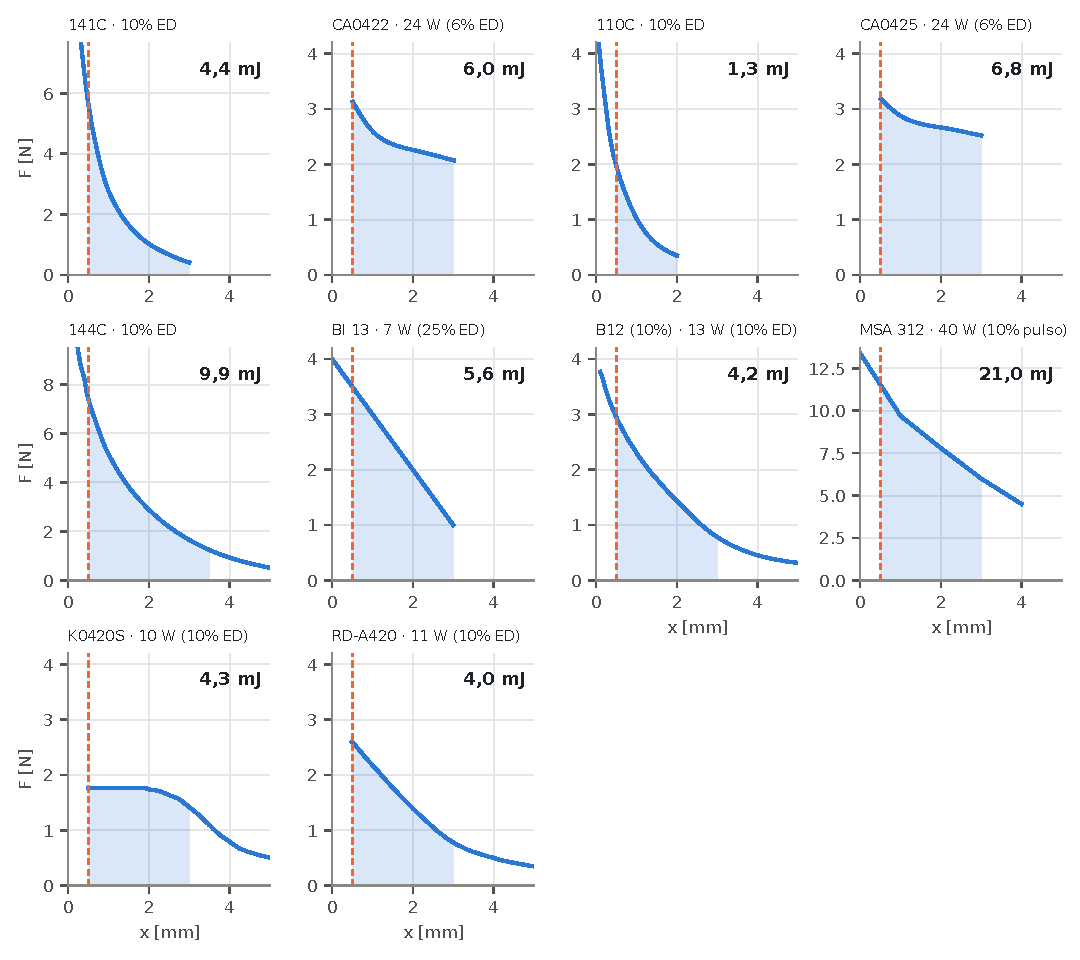
\includegraphics[width=0.8\linewidth]{fig_curvas.pdf}
  \caption{Curvas fuerza--carrera extraídas de las hojas. Sombreado: trabajo útil entre la carrera inicial y
  $x=0{,}5$~mm (línea naranja). Escalas verticales distintas.}
\end{figure}

\begin{figure}[H]\centering
  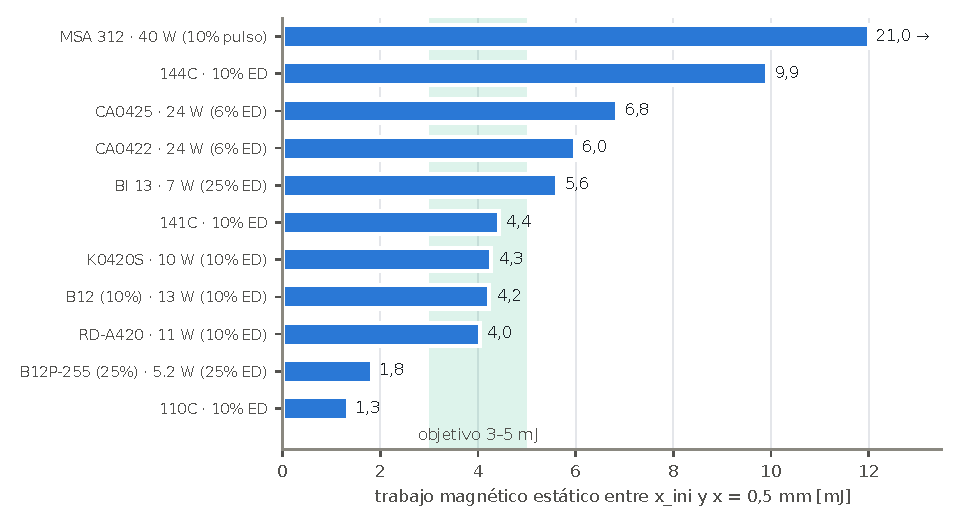
\includegraphics[width=0.9\linewidth]{fig_energia.pdf}
  \caption{Trabajo estático disponible sin llegar al tope. Franja verde: objetivo de energía cinética.}
\end{figure}

\begin{table}[H]\centering\scriptsize\setlength{\tabcolsep}{2.2pt}
\begin{tabular}{l r r r r r r r r}
\toprule
Candidato (curva) & Ventana & $W_\mathrm{útil}$ & $W$ al tope & $F_\mathrm{ini}\to F_\mathrm{imp}$ & $S_{0,1}$ & $m$ émbolo & $v_\mathrm{máx}$ & $v$ (4~mJ)\\
 & [mm] & [mJ] & [mJ] & [N] & [\%] & [g] & [m/s] & [m/s]\\
\midrule
Takaha CA0425 (24~W)        & 3,0$\to$0,5  & 6,8  & $\geq$6,8 & 2,52$\to$3,18 & 4,6  & $\approx$2,2 & 2,07 & 1,58\\
Takaha CA0422 (24~W)        & 3,0$\to$0,5  & 6,0  & $\geq$6,0 & 2,07$\to$3,13 & 5,2  & $\approx$2,0 & 2,00 & 1,63\\
Geeplus 144C (10\,\%)       & 3,5$\to$0,5  & 9,9  & 14,7 & 1,24$\to$7,41 & 7,5  & 3,0 & 2,23 & 1,41\\
Geeplus 141C (10\,\%)       & 3,0$\to$0,5  & 4,4  & 8,9  & 0,41$\to$5,66 & 12,8 & 2,5 & 1,59 & 1,51\\
Ledex B12 (13~W, 10\,\%)    & 3,0$\to$0,5  & 4,2  & 5,6  & 0,78$\to$2,95 & 7,0  & 1,4 & 1,88 & 1,83\\
Ledex B12P-255 (25\,\%)     & 2,54$\to$0,5 & 1,8  & 2,5  & 0,37$\to$1,83 & 10,0 & 1,4 & 1,24 & 1,83\\
Geeplus RD-A420 (10\,\%)    & 3,0$\to$0,5  & 4,0  & $\geq$4,0 & 0,78$\to$2,59 & 6,4 & 2,0 & 1,64 & 1,63\\
Transmotec K0420S (10~W)    & 3,0$\to$0,5  & $\geq$4,3 & -- & 1,42$\to\geq$1,77 & 4,1 & $\approx$1 & 2,07 & 2,00\\
Kendrion BI~13 (25\,\%)     & 3,0$\to$0,5  & 5,6  & 7,5  & 1,0$\to$3,5   & 6,2  & 6,0 & 1,27 & 1,07\\
MSA 312 (pulso 10\,\%)      & 3,0$\to$0,5  & 21,0 & 27,2 & 6,0$\to$11,6  & 5,5  & 7,0 & 2,29 & 1,00\\
Geeplus 110C (10\,\%)       & 2,0$\to$0,5  & 1,3  & 2,9  & 0,35$\to$1,97 & 14,8 & 1,0 & 1,15 & 2,00\\
\bottomrule
\end{tabular}
\caption{Resultados por candidato (\texttt{resultados.json}). $v$ con émbolo + 1~g de punta; $v_\mathrm{máx}$ con
$\eta=1$. «$\geq$»: la curva publicada no llega a $x<0{,}5$~mm (Takaha) o sale del gráfico (Transmotec,
recortada a 180~gf).}
\end{table}

\begin{figure}[H]\centering
  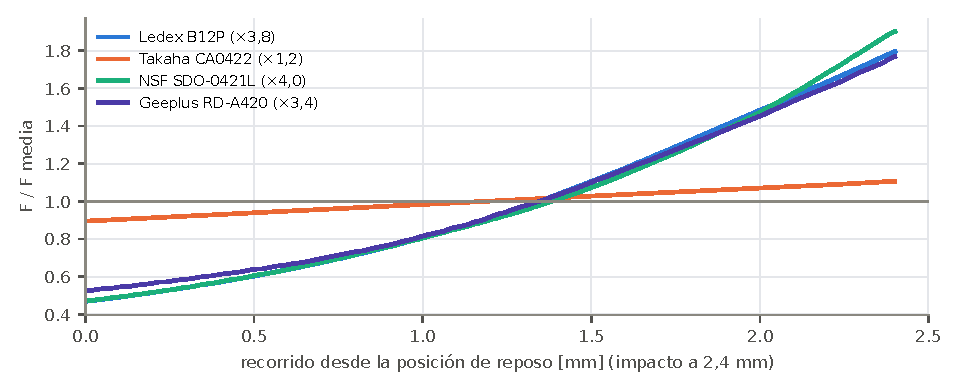
\includegraphics[width=0.9\linewidth]{fig_forma.pdf}
  \caption{Planitud en la ventana útil: el 141C multiplica su fuerza por 14 entre el inicio de carrera y el
  impacto, el 110C por 5,6 y el CA0422 por 1,5.}
\end{figure}

Los tubulares de polo cónico (Geeplus 110/141/144) concentran la fuerza cerca del tope: el último medio
milímetro guarda el \textbf{50\,\%} del trabajo en el 141C, el \textbf{54\,\%} en el 110C y el \textbf{33\,\%} en el 144C.
Como el émbolo no debe llegar al tope, esa energía no se puede usar.

%-----------------------------------------------------------------------
\section{Verificación de la preselección}
Cada dato se contrastó con la hoja del fabricante (anexo~\ref{sec:anexo}). Precios y stock al 24/09/2026.

{\footnotesize\setlength{\tabcolsep}{3pt}
\begin{longtable}{p{2.1cm} p{4.6cm} p{8.6cm}}
\toprule
Modelo & Dato de partida & Verificación\\
\midrule
\endhead
Geeplus 141C & $\varnothing$14$\times$23,4~mm & \textbf{matiz:} cuerpo $\varnothing$13,8$\times$13,7~mm; 23,4~mm es el largo con ejes.\\
 & 15~N de retención a 10\,\% ED & \textbf{matiz:} 13,4~N a 0~mm según el trazo vectorial.\\
 & «energía sobrada para 3--5~mJ» & \textbf{incorrecto:} 8,9~mJ hasta el tope, 4,4~mJ sin tocarlo.\\
 & 3~mm; 13,3~W; émbolo 2,5~g; $>$5~M & confirmado.\\
Takaha CA0422 & 9,8$\times$10,8$\times$21,3; 3/6~mm; 11~g; USD~9,11 & confirmado (hoja y tienda).\\
 & 2~N a 3~mm (6\,\%); $\approx$5--8~mJ & confirmado: 2,07~N; 6,0~mJ entre 3 y 0,5~mm.\\
 & vida «cientos de miles a millones» & \textbf{no verificable:} ni hoja ni tienda publican vida.\\
Geeplus 110C & $\varnothing$11,3$\times$19,1; 2~mm; 4,5~N; 1~g; $>$5~M & confirmado (4,8~N; cuerpo 13,3~mm de largo).\\
 & «$\approx$2--4~mJ, borderline» & \textbf{incorrecto:} 2,9~mJ al tope, 1,3~mJ sin tocarlo.\\
Takaha CA0425 & 10$\times$12$\times$24,8; 2,5~N a 3~mm; USD~9,19 & confirmado (14~g).\\
Geeplus 144C & $\varnothing$14$\times$21; 5~mm; 12~N; 3~g; $>$5~M & confirmado (12,4~N; 30,7~mm con ejes; 18~g).\\
Kendrion BI~13 & 13$\times$12$\times$26; 3~mm; 1/4~N; 7~W; 6~g & confirmado; 6~g es la armadura, el conjunto pesa 23~g.\\
 & (omitido) & \textbf{es biestable:} un imán la retiene en el tope.\\
Ledex B12P-255-B-3 & 16$\times$8,13$\times$10,16; 2,54~mm; 5,2~W; 11~s; 1,4~g & confirmado.\\
 & «familia hasta 5~M ciclos» & \textbf{matiz:} la web de Johnson Electric dice «hasta 5~M» para toda la línea; el
   catálogo 2020, «\emph{life ratings extend to 3 million cycles depending on the product size}»; el anterior,
   50\,000--100\,000 estándar. Sin cifra para el B12.\\
 & DigiKey 330~u, USD~50,71 & confirmado (plazo de fábrica 16 semanas).\\
MSA 312 & 28,5~mm; 10~mm; 6~N a 3~mm; 40~W; 7~g & confirmado; sección 19,1$\times$19,1~mm, 36~g.\\
 & «$>$1~M ciclos típico» & \textbf{no verificable:} no figura en la hoja.\\
Transmotec K0420S & 20$\times$11$\times$7,5; 0,98~N; 10~W; 10~g; 500~k & confirmado; es de enclavamiento, sin CE ni UL. Precio no verificado.\\
Geeplus RD-A420 & 21,4$\times$10,8$\times$9,8; 2~g; $>$250~k & confirmado.\\
Delta DSOS-0416-12D & 15,8$\times$7,72$\times$9,98; 1,52~mm; 100~k; EOL & medidas y carrera confirmadas (DigiKey, USD~7,38, «Active»). La hoja de Delta pide registro: vida y EOL \textbf{no verificados}.\\
\bottomrule
\end{longtable}}

%-----------------------------------------------------------------------
\section{Evaluación por candidato}
\subsection{Takaha CA0422 y CA0425}
Curva casi horizontal: aceleración uniforme y energía poco dependiente de la posición de la cuña. La curva
publicada empieza en 0,5~mm, que coincide con el punto de impacto elegido. Cinco bobinados de 24 a
384~$\Omega$; con 24~$\Omega$ a 24~V se usa la curva de 24~W (6\,\%).
\begin{itemize}
  \item \textbf{Tracción:} el émbolo entra al bastidor. Para golpear hacia afuera hay que invertir el sentido
        (palanca: agrega masa, fricción y juego), orientar el robot para golpear «hacia atrás» o pedir a Takaha
        una versión de empuje con varilla pasante. \textbf{Consultar antes de diseñar.}
  \item \textbf{Vida y masa del émbolo no publicadas;} curva «antes del calentamiento» a 20~°C; el émbolo desliza
        en el bastidor sin buje declarado.
\end{itemize}

\subsection{Geeplus 141C y 144C}
Push-pull con eje en ambos extremos: empujan directamente. Vida $>$5~M con buje especial y bore tratado
térmicamente (anexo, figura~\ref{fig:vida}); Geeplus aclara que la vida depende de la aplicación y que aumenta
con carrera corta y poca carga lateral. Aislación clase~E; respuesta $\approx$6~ms a 3~mm (141C). Geeplus
modifica émbolos y ejes en lotes chicos: \textbf{émbolo de ángulo bajo} (más fuerza en posición extendida,
aplana la curva) y \textbf{eje desacoplado por resorte} (martillo de vuelo libre).
\begin{itemize}
  \item \textbf{141C:} 4,4~mJ útiles; no alcanza 5~mJ con $\eta<1$ sin sobreexcitar; $S_{0,1}=12{,}8$\,\%.
  \item \textbf{144C:} 9,9~mJ en 3~mm, el doble de lo necesario; se regula bajando la corriente. Cuerpo
        $\varnothing$13,8$\times$21~mm, 18~g, émbolo 3~g.
\end{itemize}

\subsection{Ledex B12P}
El más compacto (16$\times$8,1$\times$10,2~mm) y con versión de empuje. Con la curva de 13~W (10\,\% ED, $\approx$19~V
para el bobinado de 27,7~$\Omega$) da 4,2~mJ. El catálogo dice que los de bastidor abierto «\emph{are typically
selected for applications in which extremely long life and precise positioning are not critical}». USD~50
contra USD~9 del Takaha.

\subsection{Descartados}
\begin{itemize}
  \item \textbf{Geeplus 110C:} 1,3~mJ; el 54\,\% del trabajo en el último medio milímetro.
  \item \textbf{Geeplus RD-A420:} misma envolvente que el CA0422 y 4,0~mJ, pero vida $>$250~k.
  \item \textbf{Kendrion BI~13:} biestable, armadura de 6~g ($v=1{,}07$~m/s para 4~mJ), 23~g; sin curva ni vida.
  \item \textbf{Transmotec K0420S:} enclavamiento, 500~k ciclos, sin CE ni UL.
  \item \textbf{MSA 312:} 21~mJ pero 19,1$\times$19,1$\times$28,5~mm y 36~g.
  \item \textbf{Delta DSOS-0416-12D:} 1,52~mm de carrera.
\end{itemize}

\subsection{Alternativa fuera de la lista: bobina móvil Geeplus VM1614}
Fuerza proporcional a la corriente y casi independiente de la posición; puede frenar o retraer invirtiendo la
corriente, así que controla la trayectoria sin topes. $\varnothing$16$\times$14~mm, 9~mm de carrera, bobina móvil de
3~g, 2,3~N de pico a 10\,\% ED, bujes de bronce sinterizado; entre 3 y 6~mm da $\approx$5~mJ. \textbf{Contras:}
$\varnothing$16~mm y cables de bobina en movimiento (verificar fatiga).

%-----------------------------------------------------------------------
\section{Decisión, ensayos y disparo}
\subsection{Matriz de decisión}
\begin{table}[H]\centering\small
\begin{tabular}{l c c c c c}
\toprule
Criterio (peso) & CA0422 & CA0425 & 141C & 144C & B12P (10\,\%)\\
\midrule
Energía útil sin tope (25\,\%)             & 4 & 4 & 2 & 5 & 2\\
Planitud / sensibilidad (20\,\%)           & 5 & 5 & 1 & 3 & 3\\
Vida declarada (20\,\%)                    & 1 & 1 & 5 & 5 & 2\\
Envolvente (15\,\%)                        & 5 & 4 & 3 & 2 & 5\\
Integración: empuje directo, guiado (10\,\%) & 2 & 2 & 5 & 5 & 4\\
Costo y disponibilidad (10\,\%)            & 5 & 5 & 3 & 3 & 3\\
\midrule
\textbf{Ponderado (sobre 5)}               & \textbf{3,65} & 3,50 & 2,95 & \textbf{3,95} & 2,95\\
\bottomrule
\end{tabular}
\end{table}
\textbf{Si la sección de 10$\times$10~mm es estricta}, 141C y 144C quedan fuera y la elección es CA0422 (sujeto a
versión de empuje y ensayo de vida) o B12P (sujeto a vida confirmada por Johnson Electric).
\textbf{Si se admite $\varnothing$14}, 144C operando en 3,5$\to$0,5~mm con corriente reducida.

\subsection{Compra para banco}
\begin{table}[H]\centering\small
\begin{tabular}{l r l l r}
\toprule
Ítem & Cant. & Bobina & Fuente & Precio ref.\\
\midrule
Takaha CA0422 & 10 & CA04220240 (24~$\Omega$: 24~W a 24~V) & takaha-japan.com & USD 9,11\\
Takaha CA0425 & 10 & CA04250240 (24~$\Omega$) & takaha-japan.com & USD 9,19\\
Geeplus 141C  & 3  & M141C-6V (19~V a 10\,\% ED) & Geeplus & cotizar\\
Geeplus 144C  & 3  & M144C-6V (19~V a 10\,\% ED) & Geeplus & cotizar\\
Ledex B12P-255-B-3 & 2 & 27,7~$\Omega$ (13~W a $\approx$19~V) & DigiKey & USD 50,71\\
\bottomrule
\end{tabular}
\end{table}

\subsection{Ensayos}
\label{sec:ensayos}
\begin{enumerate}[leftmargin=1.4em]
  \item \textbf{Energía real ($\eta$):} punta de 1~g contra yunque instrumentado; velocidad antes del contacto con
        horquilla óptica doble o láser; barrido de tensión y ancho de pulso $\to$ mapa $E(V,t_\mathrm{pulso})$.
  \item \textbf{Repetibilidad:} 1000 disparos por condición; objetivo orientativo CV$(v)<2$\,\% (CV$(E)<4$\,\%).
  \item \textbf{Sensibilidad a la posición:} correr el yunque $\pm0{,}2$~mm y contrastar con $S_{0,1}$.
  \item \textbf{Vida acelerada:} 3 unidades por modelo a 5--10~Hz hasta 5~M impactos (6--12 días); cada 500~k,
        velocidad, dispersión, juego radial y superficie del émbolo.
  \item \textbf{Temperatura:} repetir 1 con la bobina a 60--80~°C ($R$ sube $\approx$0,4\,\%/°C).
\end{enumerate}

\subsection{Electrónica de disparo}
\begin{itemize}
  \item \textbf{Driver de corriente controlada} (chopper): la energía no depende de la temperatura de la bobina ni de
        la batería del robot.
  \item \textbf{Corte antes del impacto} con apagado rápido (zéner/TVS, no diodo de libre circulación): el impactador
        llega en \textbf{vuelo libre}, sin fuerza que lo empuje contra la cuña o el tope después del contacto. El
        ancho de pulso regula la energía.
  \item \textbf{Térmica:} 24~W$\times$15~ms $=0{,}36$~J por disparo; a 1~Hz son 0,36~W, debajo de los 1,3--1,5~W
        continuos admisibles.
  \item \textbf{Velocidad:} imán en la punta y Hall doble, u horquilla óptica.
\end{itemize}

\subsection{Limitaciones}
\begin{itemize}
  \item \textbf{Curvas estáticas} de catálogo (típicas, $\pm10$\,\%): $W_\mathrm{útil}$ es cota superior; $\eta$ se mide.
  \item \textbf{Vida no publicada} para Takaha, Ledex B12 y Kendrion; la de Geeplus depende de la aplicación.
  \item \textbf{Masas estimadas} de émbolo para Takaha y Transmotec.
  \item \textbf{Precios y stock} al 24/09/2026, sin envío ni aranceles.
\end{itemize}

%-----------------------------------------------------------------------
\clearpage
\section{Anexo: hojas de datos}
\label{sec:anexo}
Páginas completas de las hojas oficiales; los recuadros rojos marcan los datos citados. Los PDF están en
\texttt{02489-00-MC005/fuentes/} (de los catálogos grandes, solo las páginas usadas). Descargas (septiembre 2026):

{\small
\begin{itemize}
  \item Geeplus, catálogo 2024 (pp.~22, 51, 54, 56--58): \url{https://www.geeplus.com/wp-content/uploads/2024/10/GEEPLUS-ELECTROMECHANICAL-ACTUATORS-CATALOGUE-2024-1.pdf}
  \item Geeplus RD-A420: \url{https://www.geeplus.com/wp-content/uploads/2019/08/Open-Frame-Solenoid_RD-A420.pdf}
  \item Takaha CA0422 / CA0425: \url{https://www.takaha.co.jp/catalog/CA0422.pdf}, \url{https://www.takaha.co.jp/catalog/CA0425.pdf}; tienda: \url{https://takaha-japan.com/products/ca0422}
  \item Ledex Open Frame DC (2020): \url{https://www.johnsonelectric.com/pub/media/image/tmp/metric-imperial/20200212_Open_Frame_DC_in_2_.pdf}; hoja B12 (RS): \url{https://docs.rs-online.com/9f8a/0900766b81634a3f.pdf}
  \item DigiKey B12P-255-B-3 y DSOS-0416-12D: \url{https://www.digikey.com}
  \item Kendrion BI~13: \url{https://www.kendrion.com/en/productfinder/group/product/linear-solenoids/bi-13-f-24v-dc-25-ed}
  \item Magnet-Schultz 312: \url{https://magnetschultz.co.uk/wp-content/uploads/312.pdf}
  \item Transmotec K0420S: \url{https://transmotec.com/Download/Datasheets/Transmotec-Datasheet-K0420S.pdf}
\end{itemize}}

\begin{figure}[H]\centering
  \hoja{0.82}{ds_takaha_CA0422.png}
  \caption{Takaha CA0422: tabla de bobinados y curva a 24~V antes del calentamiento.}
\end{figure}
\begin{figure}[H]\centering
  \hoja{0.82}{ds_takaha_CA0425.png}
  \caption{Takaha CA0425.}
\end{figure}
\begin{figure}[H]\centering
  \hoja{0.82}{ds_geeplus_141C.png}
  \caption{Geeplus push-pull 141 (catálogo 2024, p.~57): vida $>$5~M, émbolo 2,5~g.}
\end{figure}
\begin{figure}[H]\centering
  \hoja{0.82}{ds_geeplus_144C.png}
  \caption{Geeplus push-pull 144 (p.~58).}
\end{figure}
\begin{figure}[H]\centering
  \hoja{0.48}{ds_geeplus_110C.png}\hfill\hoja{0.48}{ds_geeplus_vida.png}
  \caption{Geeplus push-pull 110 (p.~56) y criterio de vida de los push-pull pequeños (p.~51).}
  \label{fig:vida}
\end{figure}
\begin{figure}[H]\centering
  \hoja{0.48}{ds_geeplus_personalizacion.png}\hfill\hoja{0.48}{ds_geeplus_VM1614.png}
  \caption{Geeplus: personalización del push-pull (p.~54; opciones 3 y 4) y bobina móvil VM1614 (p.~22).}
\end{figure}
\begin{figure}[H]\centering
  \hoja{0.48}{ds_ledex_B12.png}\hfill\hoja{0.48}{ds_ledex_B12_RS.png}
  \caption{Ledex B12: catálogo Open Frame 2020 (p.~10) y hoja del distribuidor RS. En la hoja RS, «18.» a
  0,080~in es errata de 1,8~oz.}
\end{figure}
\begin{figure}[H]\centering
  \hoja{0.48}{ds_ledex_vida.png}\hfill\hoja{0.48}{ds_geeplus_RD-A420.png}
  \caption{Ledex Open Frame, vida útil (p.~3) y Geeplus RD-A420 (vida $>$250~k).}
\end{figure}
\begin{figure}[H]\centering
  \hoja{0.48}{ds_kendrion_BI13.png}\hfill\hoja{0.48}{ds_transmotec_K0420S.png}
  \caption{Kendrion BI~13 (biestable) y Transmotec K0420S (enclavamiento, 500\,000 carreras).}
\end{figure}
\begin{figure}[H]\centering
  \hoja{0.48}{ds_msa_312.png}
  \caption{Magnet-Schultz 312: tabla de fuerza por carrera; armadura 7~g, conjunto 36~g.}
\end{figure}

\end{document}
